
\section{Dados Escalares}
	\begin{frame}{Dados Escalares}
		\begin{block}{Definição de Dado Escalar}
			Na matemática, na informática, e na física, uma \textbf{grandeza escalar} é definida quando precisamos de \textbf{um valor numérico} associado a \textbf{uma unidade de medida para caracterizar alguma grandeza}.
		\end{block}
				\pause
				\bigskip
		\begin{itemize}
			\setlength{\itemsep}{0.9em}
			\item \textit{Qual a população de Ouro Preto?}
				Cerca de 74 mil habitantes.
			\item \textit{Quantos alunos a UFOP possui?}
				Corpo Discente, são 9.658 alunos na graduação, sendo 3.363 na modalidade à distância.
				Na pós-graduação, são 434 alunos no mestrado, 121 no doutorado e 500 na especialização.
		\end{itemize}
	\end{frame}

	\begin{frame}{Dados Escalares}
		\begin{table}
			\centering
		    \begin{tabular}{c|c|c|c|c}
		    	\hline 
			    \textbf{Inscrição} & \textbf{Nota} & \textbf{Estado} & \textbf{Cidade}     & \textbf{Curso}                \\\hline \hline 
			    00467354  & 47,8 & MG     & VICOSA     & ADMINISTRACAO        \\\hline 
			    00085820  & 52,0 & MG     & UBERLANDIA & DIREITO              \\\hline 
			    00015022  & 51,0 & MG     & ALFENAS    & ENGENHARIA CIVIL     \\\hline 
			    00403068  & 08,0 & MG     & VARGINHA   & ENGENHARIA QUIMICA   \\\hline 
			    00130230  & 36,3 & MG     & UBERABA    & MEDICINA VETERINARIA \\\hline 
		    \end{tabular}
		\end{table}
	
		\begin{itemize}
			\item Com esses dados, é possível responder:
			\begin{itemize}
				\it
				\setlength{\itemsep}{1.2em}
				\item Qual a média das notas dos alunos que moram na proximidade de Uberlândia?
				\item Quais os alunos que moram numa distância maior à 300km da capital do estado?
			\end{itemize}
		\end{itemize}
	\end{frame}


\section{Dados Espaciais (Geográficos)}
	\begin{frame}{Dados Espaciais}
		\begin{table}
			\centering
			\footnotesize
		    \begin{tabular}{c|c|c|c|c|c|c}
			    \hline 
			    \textbf{Inscrição} & \textbf{Nota} & \textbf{Estado} & \textbf{Cidade}     & \textbf{Curso}                & \textbf{Latitude} & \textbf{Longitude} \\ \hline \hline 
			    00467354  & 47,8 & MG     & VICOSA     & ADMINISTRACAO        & -20.7548659        & -42.8785788         \\\hline 
			    00085820  & 52,0 & MG     & UBERLANDIA & DIREITO              & -18.9146078        & -48.2753801         \\\hline 
			    00015022  & 51,0 & MG     & ALFENAS    & ENGENHARIA CIVIL     & -21.4261129        & -45.9481612         \\\hline 
			    00403068  & 08,0 & MG     & VARGINHA   & ENGENHARIA QUIMICA   & -21.5560521        & -45.4368421         \\\hline 
			    00130230  & 36,3 & MG     & UBERABA    & MEDICINA VETERINARIA & -19.7473748        & -47.9391625         \\\hline 
		    \end{tabular}
		\end{table}
	
			\bigskip
		\begin{itemize}
			\item Com esses dados, é possível responder anteriores:
			\begin{itemize}
				\setlength{\itemsep}{1.2em}
				\it
				\item Qual a média das notas dos alunos que moram na proximidade de Uberlândia?
				\item Quais os alunos que moram numa distância maior à 300km da capital do estado?
			\end{itemize}
		\end{itemize}
	\end{frame}

	\begin{frame}{Relações entre dados e espaço}
		\begin{itemize}
			\setlength{\itemsep}{1.2em}
			\item Localização:
			\begin{itemize}
				\item Existe uma cidade chamada ``São Paulo''?
				\item Existe uma cidade em -23.5505199, -46.6333094?
			\end{itemize}
			
			\item Vizinhança:
			\begin{itemize}
				\item Qual a cidade mais próxima à São Paulo?
			\end{itemize}
			
			\item Extensão:
			\begin{itemize}
				\item Qual o perímetro de São Paulo?
				\item Qual a área de São Paulo?
			\end{itemize}
		\end{itemize}
	\end{frame}
	
	\begin{frame}
		\begin{figure}
			\centering
			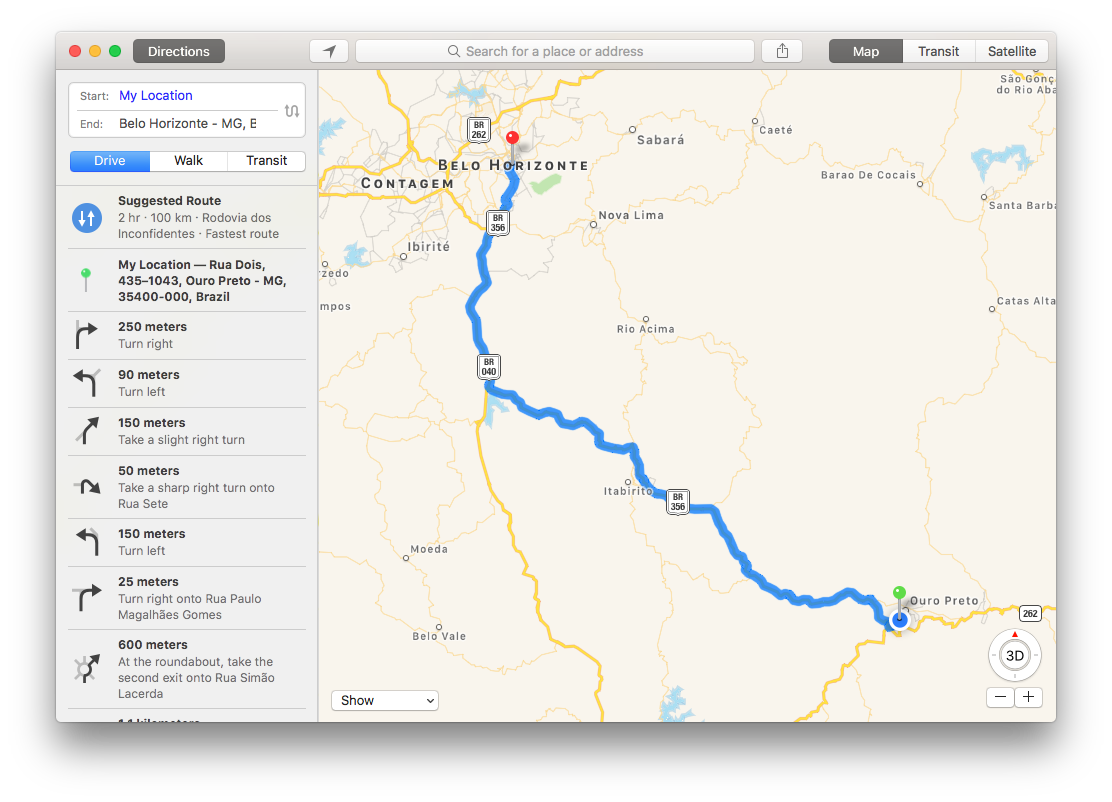
\includegraphics[width=0.80\textwidth]{img/localizacao_1.png}
		\end{figure}
	\end{frame}
	
	\begin{frame}
		\begin{figure}
			\centering
			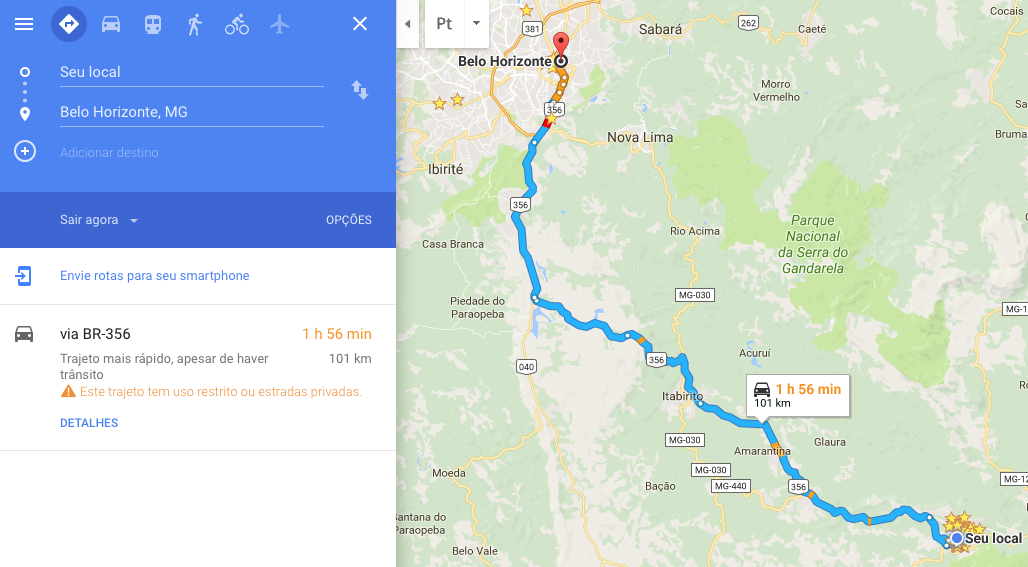
\includegraphics[width=0.90\textwidth]{img/localizacao_2.png}
			%\caption{Dados vetoriais.}
		\end{figure}
	\end{frame}
	
	\begin{frame}
		\begin{figure}
			\centering
			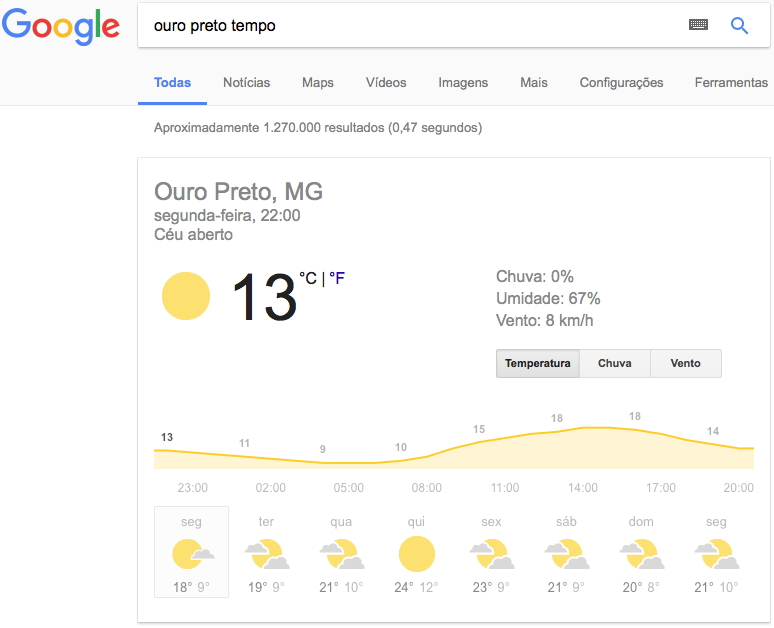
\includegraphics[width=0.7\textwidth]{img/localizacao_4.png}
		\end{figure}
	\end{frame}
	
	\begin{frame}
		\begin{figure}
			\centering
			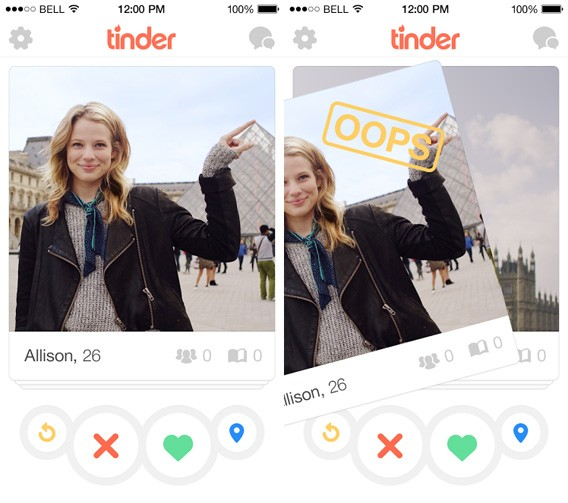
\includegraphics[width=0.65\textwidth]{img/localizacao_3.jpg}
		\end{figure}
	\end{frame}
	
	\begin{frame}
		\begin{figure}
			\centering
			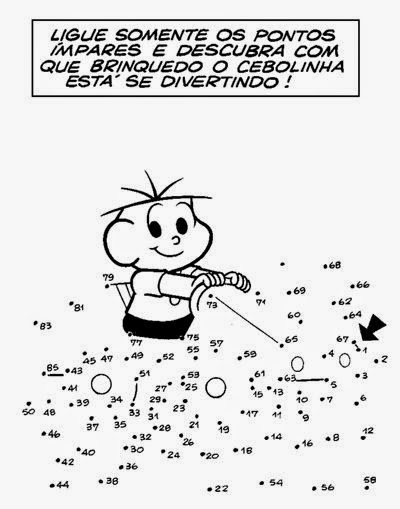
\includegraphics[width=0.42\textwidth]{img/uso_1.jpg}
		\end{figure}
	\end{frame}
	
	\begin{frame}
		\begin{figure}
			\centering
			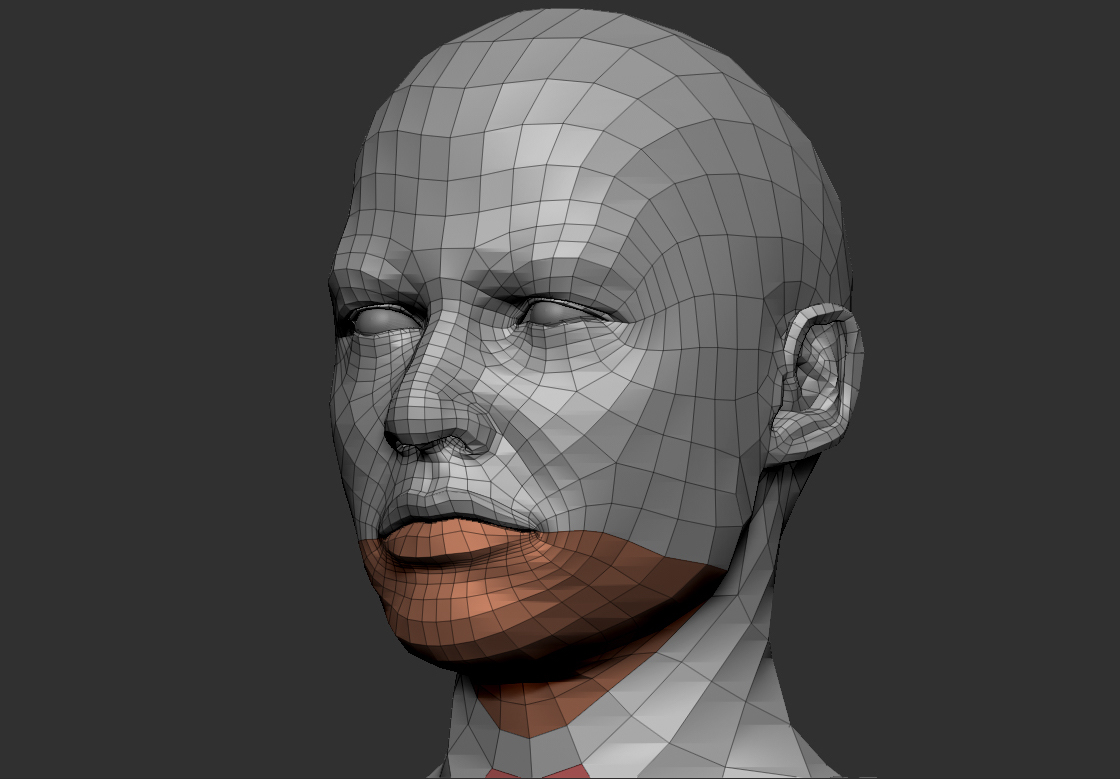
\includegraphics[width=0.72\textwidth]{img/uso_2.jpg}
		\end{figure}
	\end{frame}


\section{Banco de Dados}
	\subsection{Conceituação}
		\begin{frame}{Introdução à Banco de Dados}
			\begin{block}{Conceito}
				Banco de dados é uma coleção de dados relacionados, projetados para uma finalidade específica.
			\end{block}
				\pause
				\bigskip
			Exemplo de Banco de Dados:
			\begin{table}
				\centering
				\begin{tabular}{c|c|c|c|c}
					\hline 
					\textbf{Inscrição} & \textbf{Nota} & \textbf{Estado} & \textbf{Cidade}     & \textbf{Curso}                \\\hline \hline 
					00467354  & 47,8 & MG     & VICOSA     & ADMINISTRACAO        \\\hline 
					00085820  & 52,0 & MG     & UBERLANDIA & DIREITO              \\\hline 
					00015022  & 51,0 & MG     & ALFENAS    & ENGENHARIA CIVIL     \\\hline 
					00403068  & 08,0 & MG     & VARGINHA   & ENGENHARIA QUIMICA   \\\hline 
					00130230  & 36,3 & MG     & UBERABA    & MEDICINA VETERINARIA \\\hline 
				\end{tabular}
			\end{table}
		\end{frame}

		\begin{frame}{Aplicações de um Banco de Dados Comum}
			\begin{itemize}
				\setlength{\itemsep}{1em}
				\item \textbf{Bancos:} depósito ou retirada de fundos da conta bancária;
				\item \textbf{Hotéis:} reservas de quartervas de quartos;
				\item \textbf{Empresas aéreas:} compra e reserva de passagens;
				\item \textbf{Bibliotecas:} consulta ao acervo;
				\item \textbf{Supermercados:} identificação dos produtos comprados, controle do estoque;
				\item \textbf{Lojas virtuais:} clientes e produtos vendidos pelo site;
				\item \textbf{Redes sociais:} fotografias, postagens, curtidas, localização.
			\end{itemize}
		\end{frame}

	\subsection{Banco de Dados Espaciais}

		\begin{frame}{SGBD e BDG}
			%http://www.infoescola.com/informatica/banco-de-dados-geograficos/
			\begin{itemize}
				\setlength{\itemsep}{1em}
				\item Para gerência desses dados, utiliza-se softwares chamados \textbf{Sistemas Gerenciadores de Banco de Dados (SGBDs)}. 
				\begin{itemize}
					\item São exemplos de programas desse tipo: PostgreSQL, MySQL, Access e Oracle.
				\end{itemize}
				
				\item Requisito fundamental hoje nos SGBDs:
				\begin{itemize}
					\item Manipulação dos dados espaciais.
				\end{itemize}
				
				\item \textbf{Banco de Dados Geográficos (BDG)}\footnote{Também são chamados de \textbf{Banco de Dados Espaciais (BDE)}.}, possui o diferencial de suportar dados geométricas em suas tabelas.
	
				\item Possibilita a realização de cálculos como áreas, distâncias e centróides, além de realizar a geração de buffers (zona de influência) e outras operações entre as geometrias.
			\end{itemize}
		\end{frame}

		\begin{frame}{SGBD e BDG}
			%http://www.infoescola.com/informatica/banco-de-dados-geograficos/
			\begin{itemize}
				\item Ao construir um Banco de Dados Geográficos será possível realizar consultas tais como:
	
				\begin{itemize}
					\setlength{\itemsep}{1.2em}
					\item \textit{Que cidades são vizinhas ao município de Ouro Preto?}
					\item \textit{Que municípios são cortados pela BR-040?”}
					\item \textit{Que distância entre a comunidade rural $x$ e a escola mais próxima?”}
				\end{itemize}
			\end{itemize}
		\end{frame}

		\begin{frame}{Aplicações de um Banco de Dados Geográfico}
			%http://www.infoescola.com/informatica/banco-de-dados-geograficos/
			\begin{itemize}
				\setlength{\itemsep}{0.9em}
	
				\item Por exemplo os \textit{softwares}:
				\begin{enumerate}
					\setlength{\itemsep}{0.3em}
					\item Sistema de Informação Geográfica (Cartografia);
					\item CAD (Computer-Aided Design);
					\item Robótica;
					\item Bancos tradicionais na qual um registro com $k$ atributos corresponde a um ponto no espaço $k-d$ onde $d$ é a dimensão;
					\item Banco temporal, onde o tempo pode ser considerado uma dimensão a mais;
				\end{enumerate}

				\item Fazendo processamentos como:
				\begin{enumerate}
					\setlength{\itemsep}{0.3em}
					\item Medir distâncias, perímetro, áreas;
					\item Calcular a conectividade e o caminho mais curto entre dois pontos;
					\item Analisar pontos e linhas dentro de um polígono; 
					\item Realizar buscar por região (intervalo);
					\item etc.
				\end{enumerate}
			\end{itemize}
		\end{frame}

		\begin{frame}{Outras Aplicações}
			Fora da área de geoprocessamento, QuadTree pode ser usado em:
			\begin{itemize}
				\setlength{\itemsep}{1.5em}
				\item Fotografias e imagens;
				\begin{enumerate}
					\item Algoritmos de compressão de imagens;
					\item Correção de deformações em fotos como olhos avermelhados;
					\item Rotação de imagens.
				\end{enumerate}
				
				\item Medicina:
				\begin{enumerate}
					\item Ecografias, identificando tumores pela cor na imagem.
				\end{enumerate}
				
				\item Video-chamadas:
				\begin{enumerate}
					\item Trasmitindo somente o que foi alterado na imagem.
				\end{enumerate}
				
				\item Jogos:
				\begin{enumerate}
					\item Detecção de colisão.
				\end{enumerate}
			\end{itemize}
		\end{frame}